\documentclass{article}
\usepackage{tikz}
\usetikzlibrary{calc,3d,arrows,shapes}
\usepackage{tikz-3dplot}
\usetikzlibrary{external}
\tikzexternalize % activate!
\begin{document}



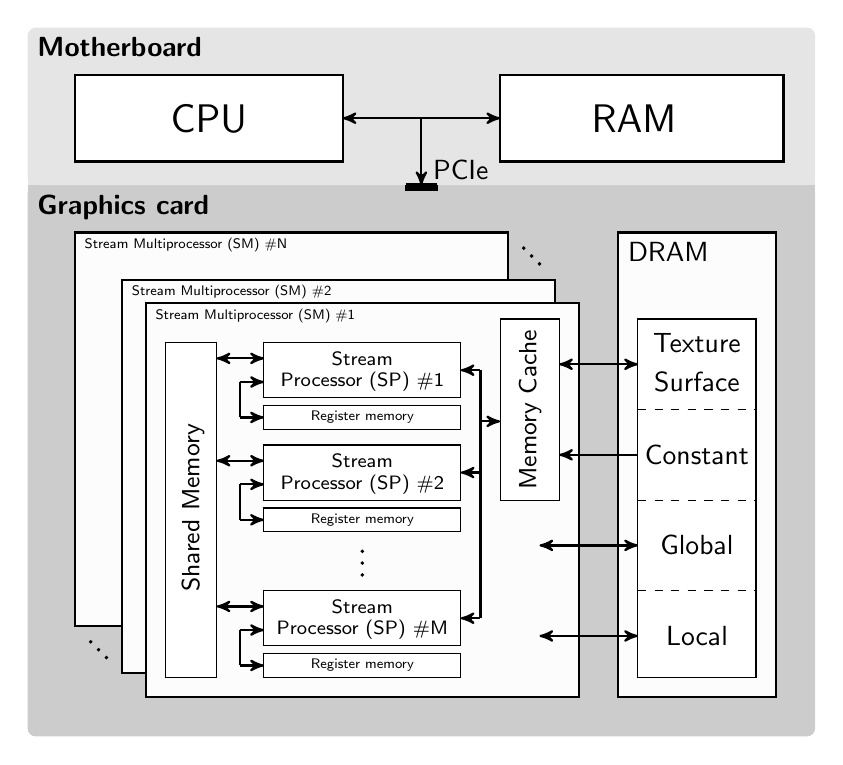
\begin{tikzpicture}[>=stealth',           % arrow tip
                    xscale=1,font=\sffamily]  


%%%% graphic card basics
\fill[rounded corners=1mm,black!20] (0,-7) rectangle (10,0); 
\fill[,black!20] (0,-1) rectangle (10,0);

\node[rotate=0,below right] at (0,0) {\textbf{Graphics card}};


%%%%motherboard basics
\fill[rounded corners=1mm,black!10] (0,0) rectangle (10,2); 
\fill[,black!10] (0,0) rectangle (10,1); 
\node[rotate=0,below right] at (0,2) {\textbf{Motherboard}};

\draw[fill=white,thick] (0.6,0.3) rectangle (4,1.4);
\node[rotate=0] at (2.3,0.85) {\Large{CPU}};


\draw[fill=white,thick] (6,0.3) rectangle (9.6,1.4);
\node[rotate=0] at (7.7,0.85) {\Large{RAM}};

 \draw[thick,<->](4,0.85) -- (6,0.85);
 \draw[thick,->](5,0.85) -- (5,0.);
 \draw[very thick](4.8,0.) -- (5.2,0.);
 \draw[fill=black](4.8,0.) rectangle (5.2,-0.07);

\node[rotate=0] at (5.5,0.2) {{PCIe}};




%%%% SMs

\draw[fill=black!1,thick] (0.6,-5.6) rectangle (6.1,-.6); 
\node[rotate=0,below right] at (0.6,-0.55) {\tiny{Stream Multiprocessor (SM) \#N}};

\draw[fill=black!1,thick] (1.2,-6.2) rectangle (6.7,-1.2); 
\node[rotate=0,below right] at (1.2,-1.15) {\tiny{Stream Multiprocessor (SM) \#2}};

\draw[fill=black!1,thick] (1.5,-6.5) rectangle (7,-1.5); 
\node[rotate=0,below right] at (1.5,-1.45) {\tiny{Stream Multiprocessor (SM) \#1}};

%etc SM
 % top right
\draw  node[fill,circle,inner sep=0.5pt,minimum size=1pt] at (6.5,-1){};
\draw  node[fill,circle,inner sep=0.5pt,minimum size=1pt] at (6.4,-0.9){};
\draw  node[fill,circle,inner sep=0.5pt,minimum size=1pt] at (6.3,-0.8){};
   % bottome left
\draw  node[fill,circle,inner sep=0.5pt,minimum size=1pt] at (1,-6){};
\draw  node[fill,circle,inner sep=0.5pt,minimum size=1pt] at (0.9,-5.9){};
\draw  node[fill,circle,inner sep=0.5pt,minimum size=1pt] at (0.8,-5.8){};

% cache

\draw[fill=white] (6,-1.7) rectangle (6.75,-4);
\node[rotate=90] at (6.38,-2.85) {\small{Memory Cache}};

%% shared
\draw[fill=white] (1.75,-2) rectangle (2.4,-6.25);
\node[rotate=90] at (2.1,-4.1) {\small{Shared Memory}};

%% SPs

\draw[fill=white] (3,-2) rectangle (5.5,-2.7);
\node[rotate=0] at (4.25,-2.2) {\scriptsize{Stream }};
\node[rotate=0] at (4.25,-2.5) {\scriptsize{Processor (SP) \#1 }};
\draw[fill=white] (3,-2.8) rectangle (5.5,-3.1);
\node[rotate=0] at (4.25,-2.95) {\tiny{Register memory}};


\draw[fill=white] (3,-3.3) rectangle (5.5,-4);
\node[rotate=0] at (4.25,-3.5) {\scriptsize{Stream }};
\node[rotate=0] at (4.25,-3.8) {\scriptsize{Processor (SP) \#2 }};
\draw[fill=white] (3,-4.1) rectangle (5.5,-4.4);
\node[rotate=0] at (4.25,-4.25) {\tiny{Register memory}};



\draw[fill=white] (3,-5.15) rectangle (5.5,-5.85);
\node[rotate=0] at (4.25,-5.35) {\scriptsize{Stream }};
\node[rotate=0] at (4.25,-5.65) {\scriptsize{Processor (SP) \#M }};
\draw[fill=white] (3,-5.95) rectangle (5.5,-6.25);
\node[rotate=0] at (4.25,-6.1) {\tiny{Register memory}};

%etc SPs

\draw  node[fill,circle,inner sep=0.5pt,minimum size=1pt] at (4.25,-4.65){};
\draw  node[fill,circle,inner sep=0.5pt,minimum size=1pt] at (4.25,-4.8){};
\draw  node[fill,circle,inner sep=0.5pt,minimum size=1pt] at (4.25,-4.95){};


%%% DRAM
\node[rotate=0,below right] at (7.5,-0.6) {{DRAM}};
\draw[fill=black!1,thick] (7.5,-6.5) rectangle (9.5,-.6); 
\node[rotate=0,below right] at (7.5,-0.6) {{DRAM}};
%memory types
\draw[fill=white] (7.75,-1.7) rectangle (9.25,-6.25);
\draw[dashed] (7.75,-2.85)--(9.25,-2.85);
\draw[dashed] (7.75,-4)--(9.25,-4);
\draw[dashed] (7.75,-5.15)--(9.25,-5.15);

\node[rotate=0] at (8.5,-2.) {{Texture}};
\node[rotate=0] at (8.5,-2.5) {{Surface}};

\node[rotate=0] at (8.5,-3.425) {{Constant}};
\node[rotate=0] at (8.5,- 4.575) {{Global}};
\node[rotate=0] at (8.5,-5.725) {{Local}};



%% ARROWS
\draw[thick,<->](6.75,-2.275) -- (7.75,-2.275);
\draw[thick,<-](6.75,-3.425) -- (7.75,-3.425);

\draw[thick,<->](6.5,-4.575) -- (7.75,-4.575);
\draw[thick,<->](6.5,-5.725) -- (7.75,-5.725);

\draw[thick,<-](5.5,-2.35) -- (5.75,-2.35);
\draw[thick,<-](5.5,-3.65) -- (5.75,-3.65);
\draw[thick](5.75,-2.35) -- (5.75,-5.5);
\draw[thick,<-](5.5,-5.5) -- (5.75,-5.5);

\draw[thick,->](5.75,-3) -- (6,-3);

%register
\draw[thick](2.7,-6.1) -- (2.7,-5.65);
\draw[thick,->](2.7,-6.1) -- (3,-6.1);
\draw[thick,->](2.7,-5.65) -- (3,-5.65);

\draw[thick](2.7,-4.25) -- (2.7,-3.8);
\draw[thick,->](2.7,-4.25) -- (3,-4.25);
\draw[thick,->](2.7,-3.8) -- (3,-3.8);

\draw[thick](2.7,-2.95) -- (2.7,-2.5);
\draw[thick,->](2.7,-2.95) -- (3,-2.95);
\draw[thick,->](2.7,-2.5) -- (3,-2.5);
% shared
\draw[thick,<->](3,-2.2) -- (2.4,-2.2);
\draw[thick,<->](3,-3.5) -- (2.4,-3.5);
\draw[thick,<->](3,-5.35) -- (2.4,-5.35);



\end{tikzpicture}



















\end{document}